\setlength{\footskip}{8mm}

\chapter{Introduction} 

\textit{In this inaugural chapter, we embark on a comprehensive exploration of the intricate domain of text detection in natural scenes. This chapter serves as the gateway to our thesis, providing an essential foundation for the research that follows. Here, we set the stage, define our objectives, and establish the context for the critical challenges we aim to address. The introduction begins with an overview of the vast landscape of scene text detection, highlighting its importance and real-world applications. We then narrow our focus to the specific motivations behind our research, including the pressing need for Urdu text detection. The chapter also outlines the problem statement that drives our investigation, laying the groundwork for the subsequent chapters. In essence, this introduction sets the trajectory for our academic journey, guiding readers into the heart of our thesis and the compelling world of text detection in natural scenes.}

\section{Overview}

The landscape of scene text detection is expansive, finding applications in diverse domains such as online education, product search, and video scene parsing. Thanks to the rapid advancements in deep learning, text detection methods have exhibited impressive prowess, particularly in scenarios where text instances conform to regular shapes and aspect ratios. However, the recent research focus has gravitated toward the formidable realm of arbitrary shape text detection, which holds the promise of versatility in real-world applications. This evolution responds to the complex demands of arbitrary shaped, multi-oriented text, and the intricate backdrop of scenes with diverse and challenging backgrounds.

In our research, we hone our gaze on the intricate nuances presented by arbitrary shaped, multi-oriented text, set against the backdrop of complex scene backgrounds. Despite the notable advancements in arbitrary shape text detection a multitude of challenges continues to loom large. These challenges, arising from the inherent diversity in shapes, textures, and scales within scene texts, act as the driving force 
9
Chapter 2propelling our research endeavors. The ascent of segmentation-based methodologies marks a pivotal juncture in the domain of arbitrary shape text detection. These innovative approaches leverage pixel-level predictions to pinpoint text regions, bolstering the system's resilience against the vagaries of shape variations and intricate backgrounds. However, within this promising expanse, two paramount challenges beckon for further exploration and innovation.

% Human monitoring is therefore becoming
% increasingly expensive and ineffective as the torrent of video data
% increases. For instance, in a CCTV monitoring room (see
% Figure \ref{fig:monitoring}), security operators are required to
% monitor 24 hours a day and be ready to take action when an alarm
% occurs. 

% \begin{figure}[t]
%   \centering
%   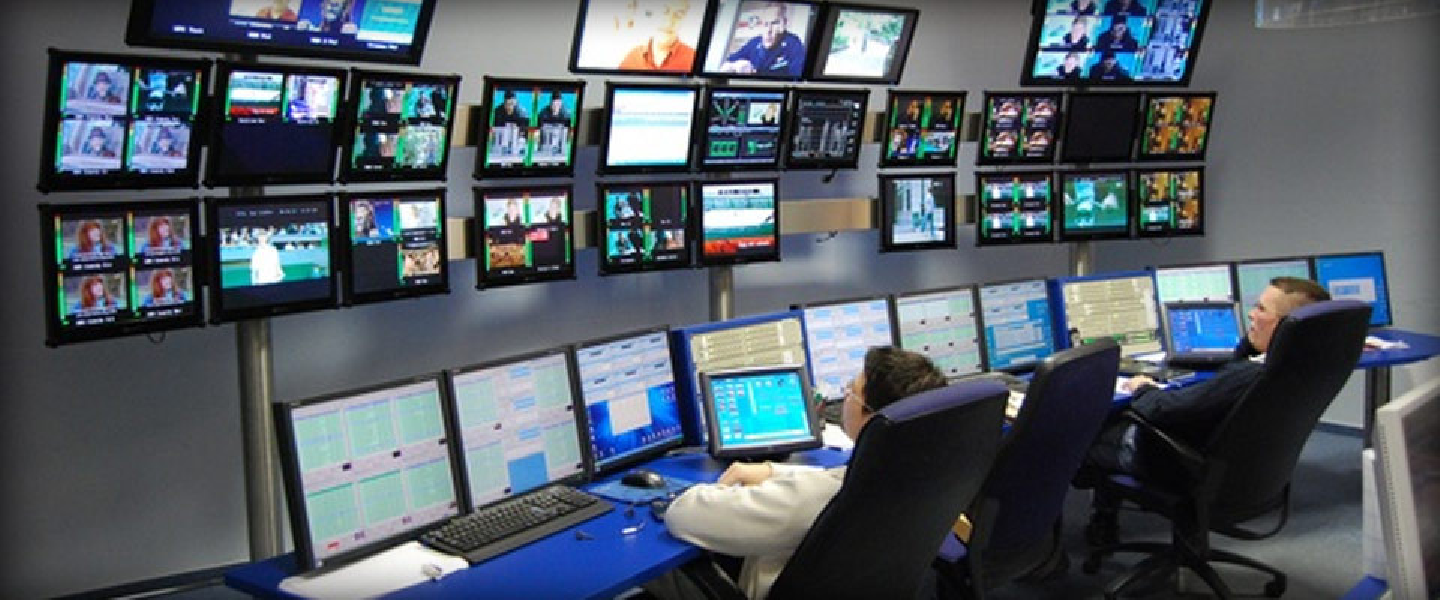
\includegraphics[width=5in]{figures/monitoring}
%   \caption[CCTV monitoring room.]{\small CCTV monitoring
%     room. Reprinted from the Twenty First Security Web site
%     (\url{http://www.twentyfirstsecurity.com.au/}).}
%   \label{fig:monitoring}
% \end{figure}

\section{Motivation}
Text extraction from natural scenes, with a particular focus on arbitrary-shaped, multi-oriented text, and text embedded within complex backgrounds, represents a pivotal challenge in the domain of computer vision. This challenge arises from the diverse and intricate nature of text within such scenes. While text detection in controlled environments, like scanned documents, has achieved remarkable accuracy, the inherent complexities of text in natural scenes introduce unique hurdles. These challenges are multifaceted and include issues such as sensor noise, blurriness, varying resolutions, non-planar text, complex layouts, inconsistent lighting, and text presented at arbitrary angles or undergoing distortion.

As technology becomes increasingly intertwined with our daily lives, the applications of robust text detection are expanding significantly. Our work is motivated by the real-world utility of accurate text extraction, as evidenced by its relevance in several key domains.

\textbf{Autonomous Devices:} The era of autonomous devices, including self-driving cars and drones, hinges on the accurate interpretation of text from road signs and traffic signals. This aspect is critical for enhancing the safety and navigational capabilities of these devices.

\textbf{Translation for Foreign Tourists:} Facilitating the translation of text from signs, menus, and documents empowers foreign tourists and fosters cross-cultural interactions. Our research aims to streamline these experiences by enhancing text extraction techniques.

\textbf{Script Identification:} Embracing the rich tapestry of world languages and scripts is an essential aspect of text detection. Preserving and recognizing diverse scripts, from Latin to Cyrillic, is integral to our research agenda.

\textbf{Geo-Localization:} Geographic Information Systems (GIS) rely on text extraction to decipher location-based data. Our research contributes to the development of GIS applications for precise mapping, urban planning, and location-specific services.

\textbf{Product Label Recognition:} Empowering consumers to scan and comprehend product labels bolsters their purchasing decisions. Our work advances technology in the realm of product label reading, contributing to a seamless shopping experience.

\textbf{Understanding ATM Machine Instructions:} ATM machines often present instructions in foreign languages, challenging users to understand them. Our research endeavors to improve text extraction, ensuring that users can access ATM services regardless of the language used.

This array of real-world applications underscores the critical role of text detection in simplifying tasks, enhancing accessibility, and elevating various domains. Our motivation is deeply rooted in a commitment to making this technology not only accurate and efficient but also broadly accessible and practical in diverse scenarios.

\subsection{The Need for Urdu Text Detection:}
Focusing on Urdu, a major South Asian language, provides a compelling case for our research. With over 170 million speakers, Urdu is one of the most prevalent languages globally, serving as Pakistan's national language and extensively spoken in India. The urgency for effective Urdu text detection becomes evident given this widespread usage. Effective technology in this context transcends language barriers, fostering cross-cultural communication and expanding opportunities for millions of Urdu speakers. It plays a pivotal role in script identification, multilingual translation, cultural preservation, and improving access to vital information. Our focus on Urdu text detection epitomizes our broader mission: extending the benefits of text detection to languages and regions where it can make a significant and positive impact.

\section{Problem Statement}
However, it's important to note that the landscape of scene text is far from uniform. Unlike the structured fonts typically found in documents, scene text is remarkably diverse. It varies in shape, orientation, texture, scale, and often appears against complex backgrounds. These inherent diversities necessitate the development of innovative text detection techniques capable of seamlessly adapting to a wide array of scenarios. Notably, the challenges posed by complex backgrounds are a critical aspect. Scene text frequently occurs in settings with backgrounds that can confound detection models. These backgrounds may include intricate urban environments or bustling marketplaces. Inconsistent lighting conditions, stemming from factors like variable weather or diverse lighting sources, further compound the complexities. The presence of occluded text, often hidden by objects or other text elements, presents a significant puzzle for detection models. Blurred text, whether due to motion or low image resolution, adds to the intricacies of text extraction. These multifaceted challenges are at the heart of our research efforts, pushing the boundaries of text detection capabilities in natural scenes. Figure ~\ref{fig:complex} provides a visual representation of these diverse and demanding conditions encountered in scene text, underscoring the compelling need for innovative solutions in this domain. 

\begin{figure}[htp]
  \centering
  \begin{minipage}{0.4\textwidth}
    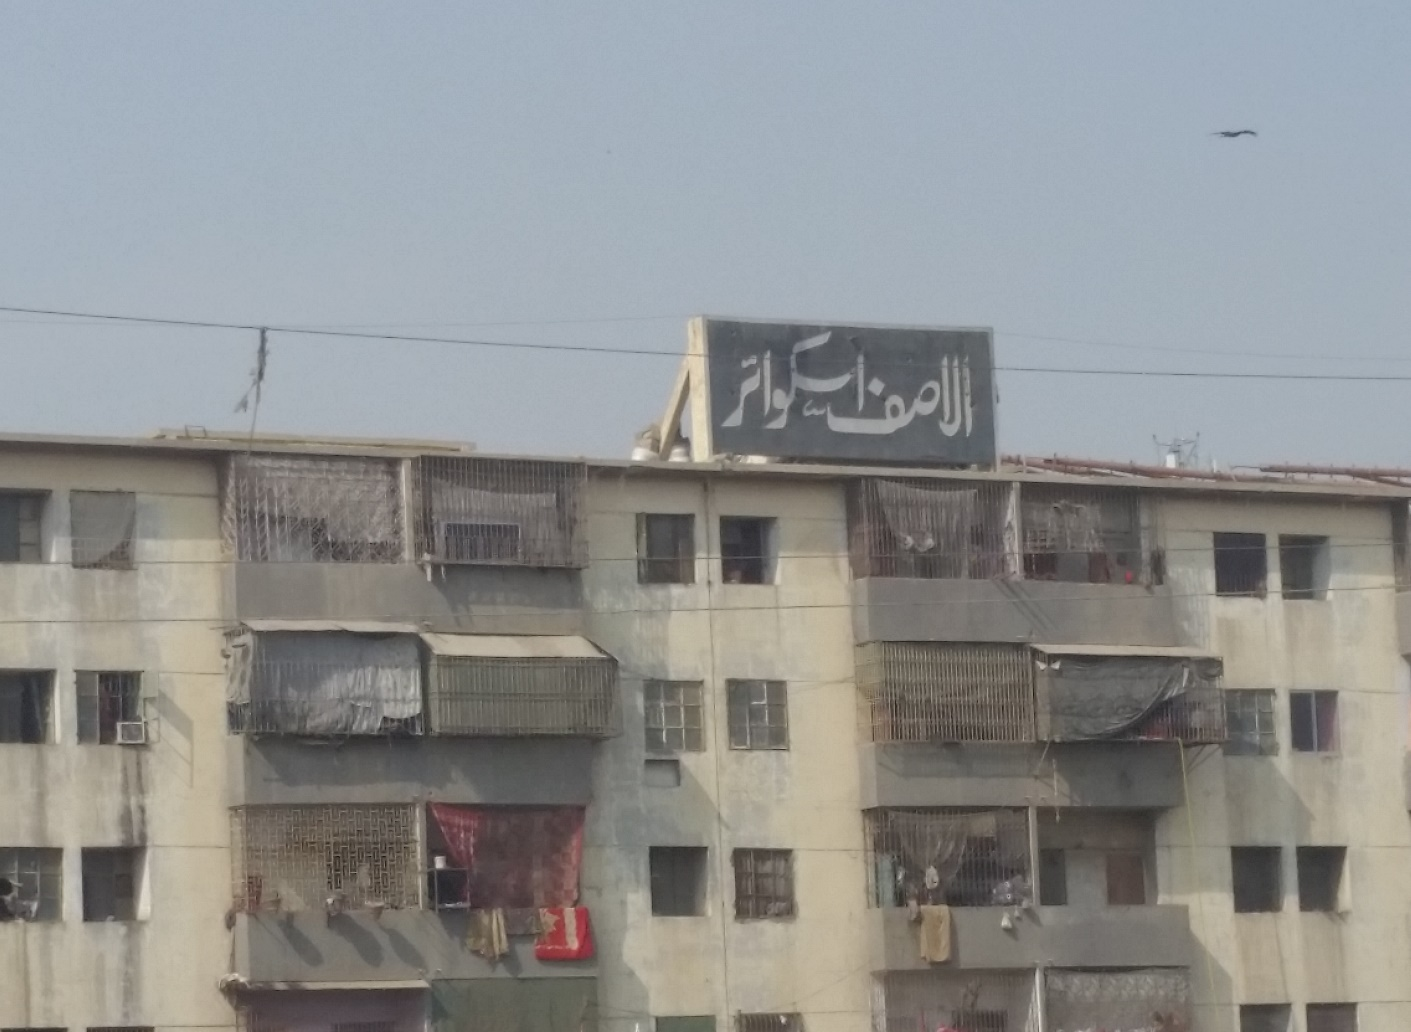
\includegraphics[width=\linewidth]{ITU-Thesis-LaTeX-Template-Updated/figures/img_998.jpg}
    \text{Complex Confusing Background}
  \end{minipage}
  \begin{minipage}{0.4\textwidth}
    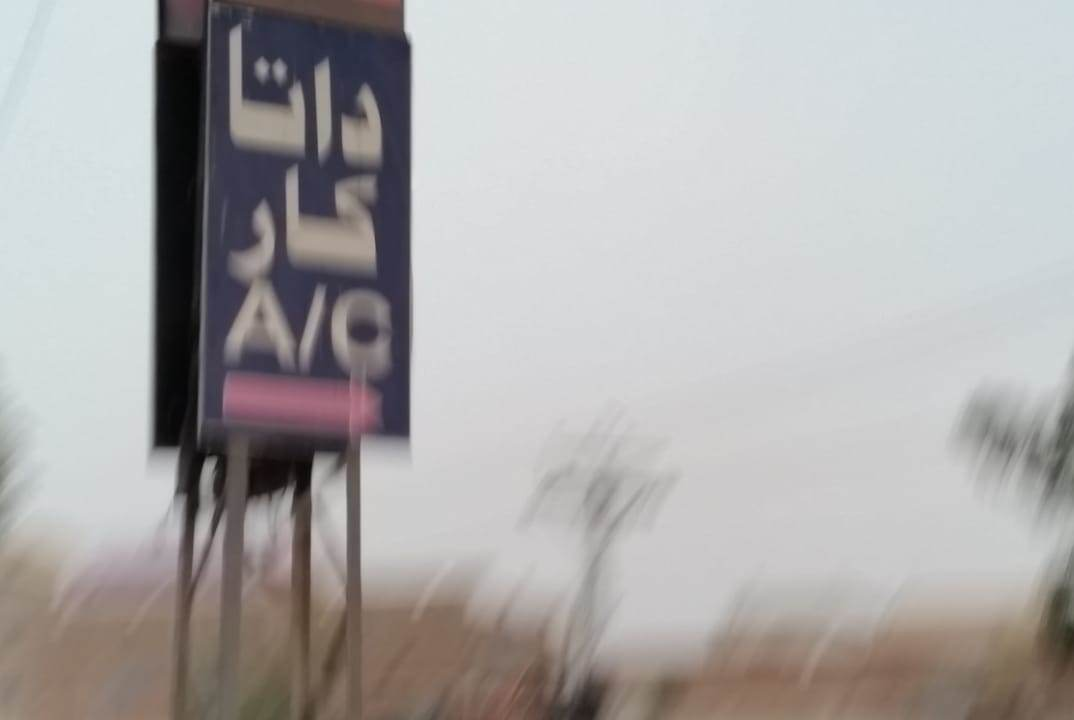
\includegraphics[width=\linewidth]{ITU-Thesis-LaTeX-Template-Updated/figures/img_783.JPG}
    \text{Blurred}
  \end{minipage}
  \begin{minipage}{0.4\textwidth}
    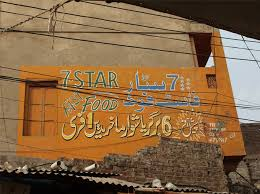
\includegraphics[width=\linewidth]{ITU-Thesis-LaTeX-Template-Updated/figures/occluded.jpg}
    \text{Occluded Text}
  \end{minipage}
  \begin{minipage}{0.4\textwidth}
    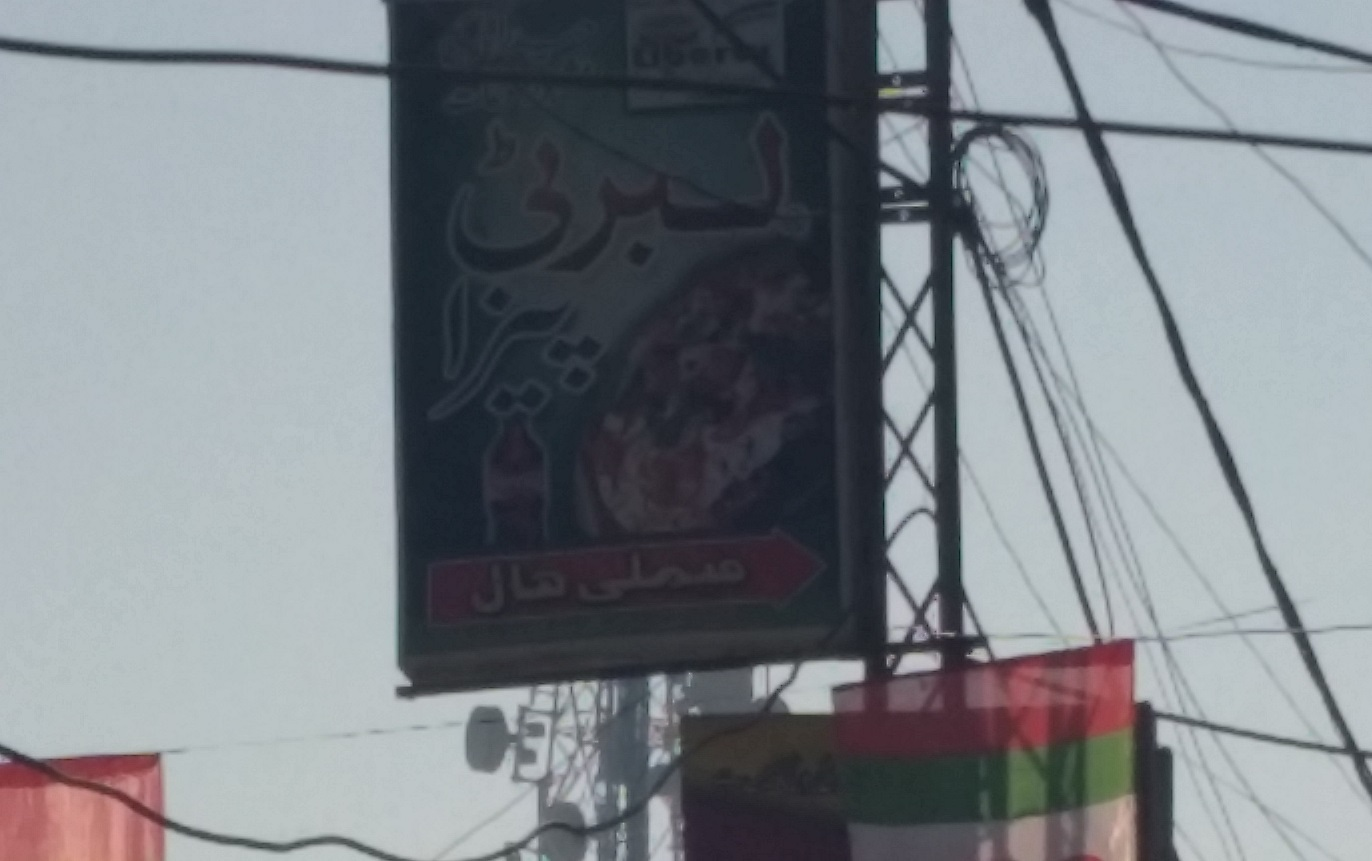
\includegraphics[width=\linewidth]{ITU-Thesis-LaTeX-Template-Updated/figures/img_1000.jpg}
    \text{Poor Lighting Condition}
  \end{minipage}
  \caption[Complex Scene Scenarios]{Complex Scene Scenarios}
  \label{fig:complex}
\end{figure}
\FloatBarrier

At the forefront of this diversity lies our primary research focus: the accurate detection of Urdu text within complex scenes. Urdu, a prominent South Asian language, serves as Pakistan's national language and is widely spoken in India, encompassing over 170 million speakers. It stands as one of the most prevalent languages worldwide. The unique challenges presented by Urdu script, which is cursive in nature, ligature-based, written from right to left, and possesses two distinct writing styles: Naskh and Nastaleeq make its accurate detection particularly demanding. This is shown in Figure ~\ref{fig:styles}.

\begin{center}
   \begin{figure}[htp]
       \centering  
        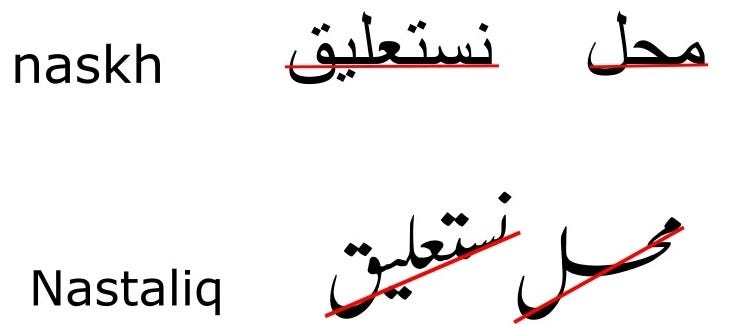
\includegraphics[width=6cm]{ITU-Thesis-LaTeX-Template-Updated/figures/urdu styles.jpg}
        \caption[Urdu writing Styles]{Urdu writing Styles}
        \label{fig:styles}
    \end{figure}
\end{center}
\FloatBarrier

This complex nature of Urdu script detection in the context of complex backgrounds is a major challenge that requires novel and innovative solutions. Despite the tremendous potential of text detection to enhance the safety, accessibility, and cross-cultural communication, there remains a dearth of suitable datasets for training models, especially for scripts like Urdu.

Our research is laser-focused on addressing these pivotal challenges, with a primary emphasis on the accurate detection of Urdu language text within intricate scene images. This problem statement encapsulates the pressing need to develop cutting-edge techniques that cater to the unique demands of scene text detection, especially within the context of complex backgrounds and challenging scripts like Urdu. Our aim is to bridge these technological gaps and facilitate the seamless integration of text detection into a wide range of real-world applications, ultimately advancing safety, accessibility, and cross-cultural interaction.
\section{Objectives}

\paragraph{Develop Robust Urdu Text Detection Algorithms:} \hfill \break
The foremost objective of this research is to advance the state-of-the-art in text detection, with a specific focus on the Urdu script. We aim to develop algorithms that can accurately locate and extract Urdu text within complex scene images, addressing challenges such as cursive nature, diverse writing styles (Naskh and Nastaleeq), and text variations.

\paragraph{Enhance Multi-Oriented and Arbitrary Shape Text Detection:} \hfill \break
Beyond Urdu, this research seeks to contribute to the broader field of text detection by enhancing the detection of multi-oriented and arbitrary-shaped text in complex backgrounds. Our algorithms should be versatile, capable of handling text in various languages and scripts.

\paragraph{Improve Scene Text Detection for Real-World Applications:} \hfill \break
We aim to create technologies that are not confined to the laboratory but are practical for real-world applications. Our research focuses on improving text detection for a range of applications, from aiding visually impaired individuals to enhancing autonomous devices and aiding in urban planning and mapping.

\section{Contributions}
\paragraph{1. Dataset Generation:} \hfill \break
A pivotal contribution of this research involves the meticulous creation of polygonal annotations for the Urdu benchmark dataset. By delineating text regions with precise polygons, we've developed a dataset that ensures a more effective and fine-grained representation of text. This dataset transcends traditional bounding boxes, enabling a closer and more accurate pixel-level capture of text instances. It empowers our algorithms to discern text with greater precision and cater to the nuanced characteristics of Urdu script.

\paragraph{2. Architecture for Enhanced Text Detection:} \hfill \break This research introduces a cutting-edge architectural paradigm for text detection, featuring a two-pronged approach: the Boundary Proposal Model and the Adaptive Deformation Model. Overview of my methodology can be seen in the Figure~\ref{fig:architecture}. In the Boundary Proposal Model, we adeptly extract crucial features encompassing classification, distance, and direction fields. These features serve as the foundational building blocks for the Adaptive Deformation Model. This latter model, constructed with an encoder-decoder structure enhanced by Graph Convolutional Networks (GCNs) and Bi-LSTM, takes text detection to new heights. It adeptly handles the intricate nuances of Urdu text, including its cursive nature and variations in shape. This innovation is set to significantly enhance text detection capabilities, not only for Urdu but also for multi-oriented and arbitrary-shaped text in complex scenes.

\begin{center}
   \begin{figure}[htp]
       \centering  
        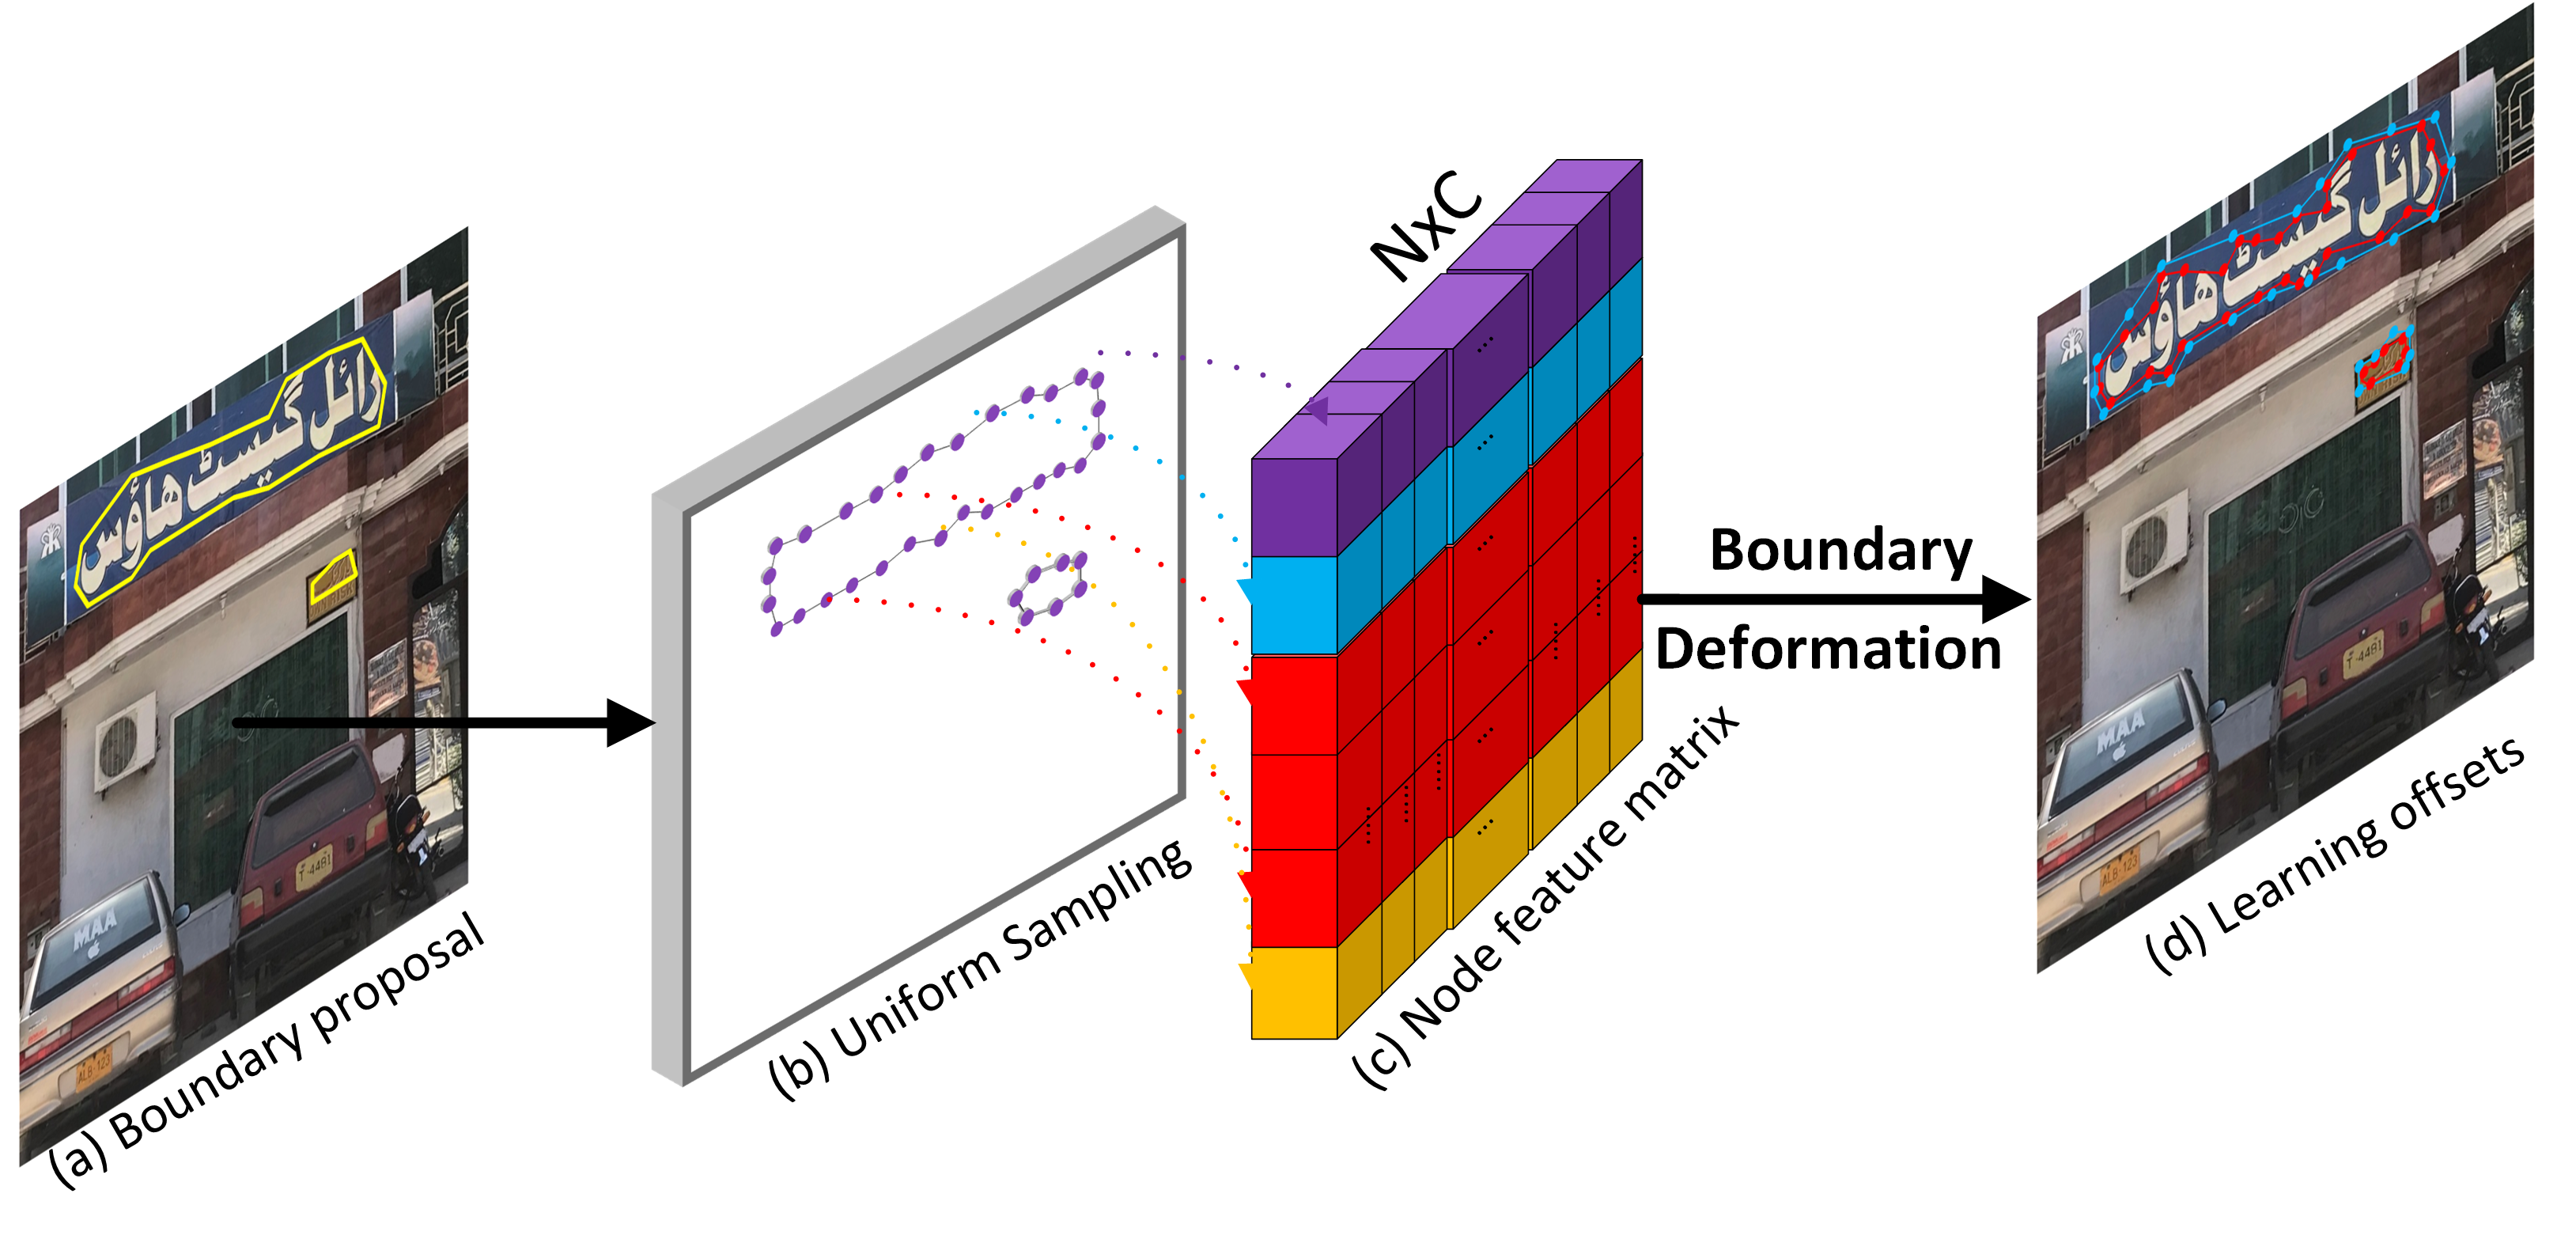
\includegraphics[width=10cm]{ITU-Thesis-LaTeX-Template-Updated/figures/Boundary Proposal Deformation HQ.png}
        \caption[Architecture Overview]{Architecture Overview}
        \label{fig:architecture}
    \end{figure}
\end{center}
\FloatBarrier

These contributions collectively advance the domain of text detection, promising more robust and precise results while providing the potential to extend their impact to the broader spectrum of text detection challenges.

\section{Limitations and Scope}
In this section, we outline the limitations and the expansive scope of our research, defining the boundaries of our study and highlighting its broader implications.

\subsection{Scope}
\paragraph{1. Urdu Text Detection:} \hfill \break
The primary scope of this research is to develop robust algorithms and methodologies for the accurate detection of Urdu text within complex scene images. This focus ensures a comprehensive exploration of challenges specific to the Urdu script.

\paragraph{2. Advanced Architecture:} \hfill \break
The research scope encompasses the innovative architecture, combining the boundary proposal model and adaptive deformation model. This architecture provides a foundation for the development of effective text detection solutions, emphasizing complex backgrounds and cursive script styles.

\paragraph{3. Real-World Applications:} \hfill \break
The developed algorithms and methodologies are designed to be practical and applicable in real-world scenarios. The scope extends to diverse applications, including aiding visually impaired individuals, enhancing the capabilities of autonomous devices, facilitating urban planning, mapping, and improving the accessibility of information.

\paragraph{4. Multilingual Potential:} \hfill \break
While the primary focus is on Urdu, the research scope acknowledges the potential for multilingual text detection. The methodologies can be adapted and expanded to cover a broader range of languages and scripts.

\paragraph{5. Dataset Generation:} \hfill \break
A significant aspect of the research scope includes the creation of comprehensive datasets, particularly for the Urdu script. This contributes to the development of benchmarks and resources for evaluating text detection algorithms.

\paragraph{6. Cross-Domain Collaboration:} \hfill \break
Collaboration with experts from various domains, including computer vision, linguistics, and artificial intelligence, is encouraged to broaden the scope of research and explore innovative solutions.

The scope of your research is dynamic and adaptable, with implications that extend beyond a single language or script. It addresses challenges unique to Urdu text detection while offering potential for broader applications and advancements in the field of text detection.

\subsection{Limitations}
This research's algorithms and models may face limitations when applied to highly complex images characterized by severe blurring, significant occlusions, and extremely inconsistent and poor lighting conditions. Such extreme scenarios can pose challenges to accurate text detection.
While the research strives to tackle a wide range of real-world challenges, it's essential to recognize the constraints and complexities introduced by highly degraded images. These limitations serve as opportunities for further exploration and refinement in the field of text detection.

\subsection{Limitations}
This research's algorithms and models may face limitations when applied to highly complex images characterized by severe blurring, significant occlusions, and extremely inconsistent and poor lighting conditions. Such extreme scenarios can pose challenges to accurate text detection.
While the research strives to tackle a wide range of real-world challenges, it's essential to recognize the constraints and complexities introduced by highly degraded images. These limitations serve as opportunities for further exploration and refinement in the field of text detection.


\pagebreak

\section{Thesis Outline}

I organize the rest of this dissertation as follows.

In Chapter \ref{ch:literature-review}, we describe the literature review.

In Chapter \ref{ch:Dataset}, we discussed how we created dataset specific to our framework

In Chapter \ref{ch:methodology}, we propose our methodology.

In Chapter \ref{ch:results}, we present the experimental results.

Finally, in Chapter \ref{ch:conclusion}, we conclude our thesis.

\FloatBarrier

